\section{Introduction}

Digital Twin (DT) technology represents the creation of a virtual replica of a physical object or system that is used to simulate, monitor, and optimize its real-world counterpart. DTs integrate real-time data from the physical entity, utilizing advanced simulation, machine learning, and reasoning techniques to enhance decision-making and operational efficiency.\cite{jiang2021industrial}
Efforts to advance the key technologies that underpin the primary capabilities of mirroring, shadowing, and threading are actively progressing in DT-driven industries. These capabilities are critical for the effective deployment and utilization of digital twins in various sectors.\cite{jiang2021industrial}
\\ \textbf{Mirroring} involves the creation of an exact virtual replica of a physical object or system in real-time. This capability is essential for applications such as real-time monitoring and diagnostics, virtual prototyping, and pre-production testing of products. Industries such as manufacturing, healthcare, and aerospace benefit significantly from precise replication and analysis, which ensures quality and efficiency in their operations.\cite{jiang2021industrial}
\\ \textbf{Shadowing} focuses on continuously updating the digital twin with real-time data from its physical counterpart. This real-time data integration is vital for predictive maintenance, real-time performance optimization, and condition monitoring. Sectors like energy, utilities, and smart cities leverage shadowing to maintain system efficiency and predict potential failures, thereby avoiding downtime and reducing maintenance costs.\cite{jiang2021industrial}
\\ \textbf{Threading} entails the integration and synchronization of multiple digital twins across different systems and processes. This capability is crucial for complex system simulations, supply chain management, and coordinated operations across multiple locations. Industries such as logistics, large-scale manufacturing, and integrated urban infrastructure rely on threading to coordinate various elements seamlessly, ensuring smooth and efficient operations.\cite{jiang2021industrial}
\\ In summary, the principles of mirroring, shadowing, and threading are fundamental to the key use cases and applications of digital twin technology. These concepts enable comprehensive and integrated approaches to monitoring, optimizing, and managing complex systems across a wide range of industries.

\begin{figure}[h]
    \centering
    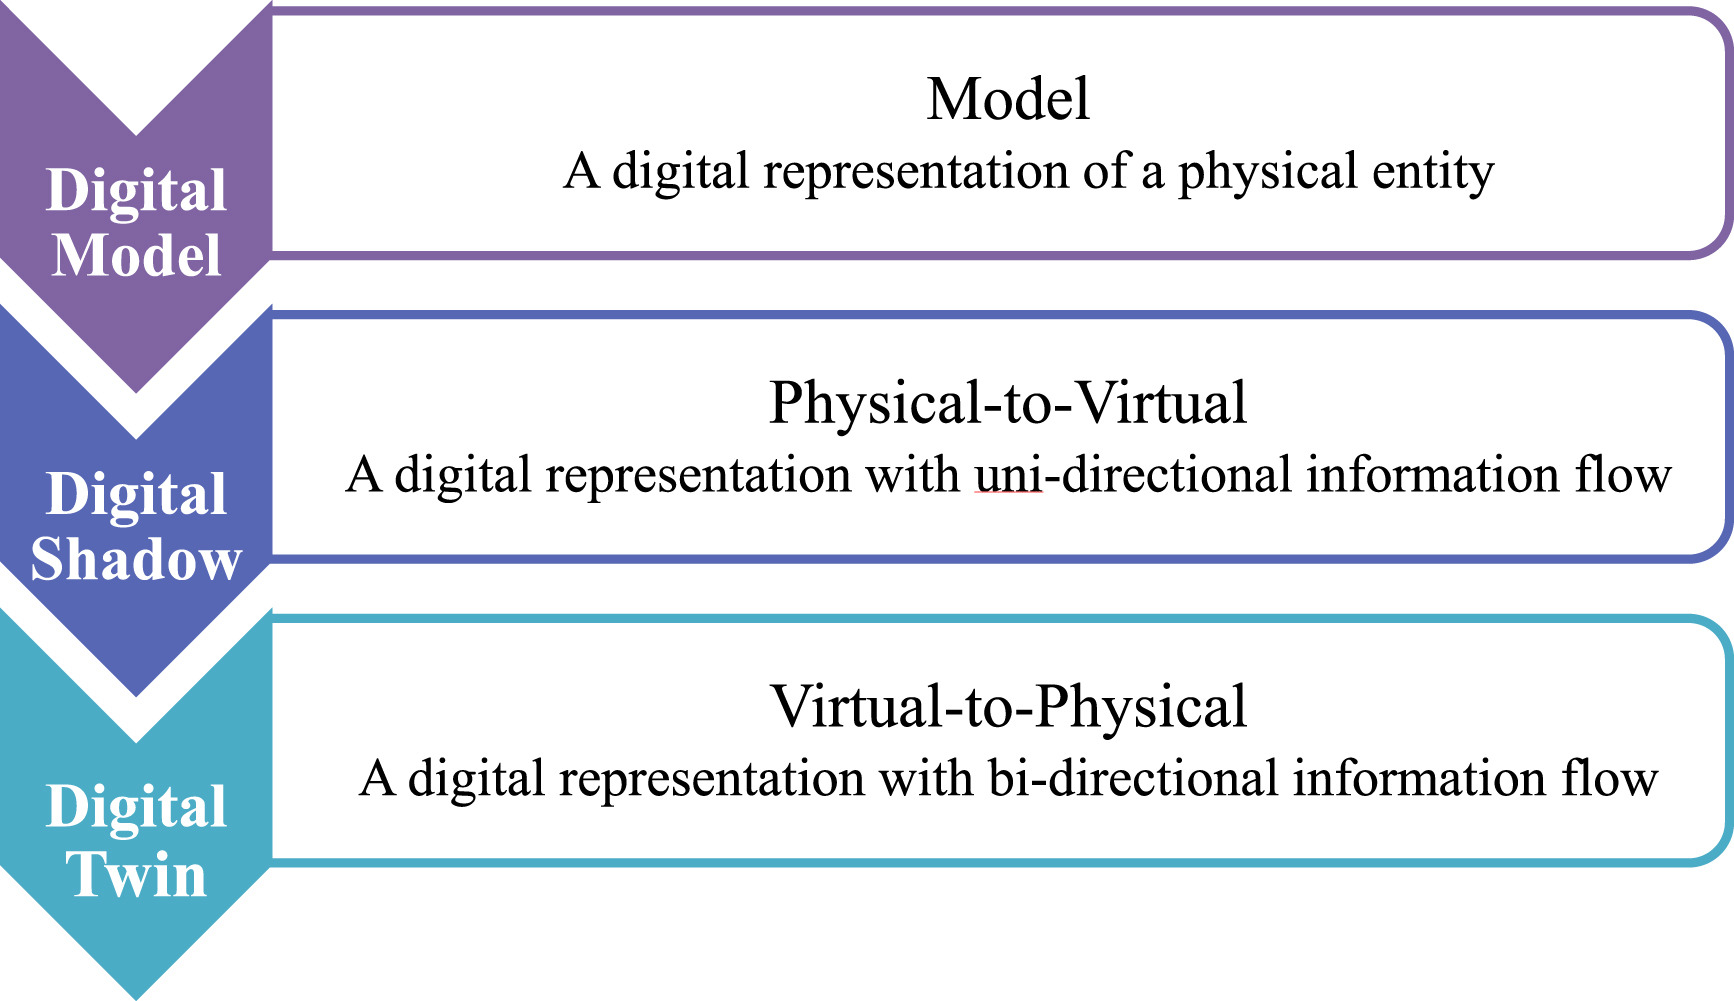
\includegraphics[width=0.6\textwidth]{DT_Layers}
    \caption{Levels of integration}
    \label{fig:mesh1}
\end{figure}